Finite State Machine (FSM) is a model for designing sequential logic circuits,
where the circuit's behavior is determined by a finite number of states, inputs and outputs.
In this case, the FSM is designed to implement \textit{five} different operations,
namely RESET, XNOR, NAND, SUB, and ADD on two 4-bit inputs A and B.
The way we coded the Verilog code represents the implementation of the FSM,
which is designed to perform the above-mentioned arithmetic and logical operations on the given input values.
From an high level perspective, The \textbf{FSM} has Four states, which are encoded as 2-bit values, as follows:

\begin{figure}[H]
    \centerline{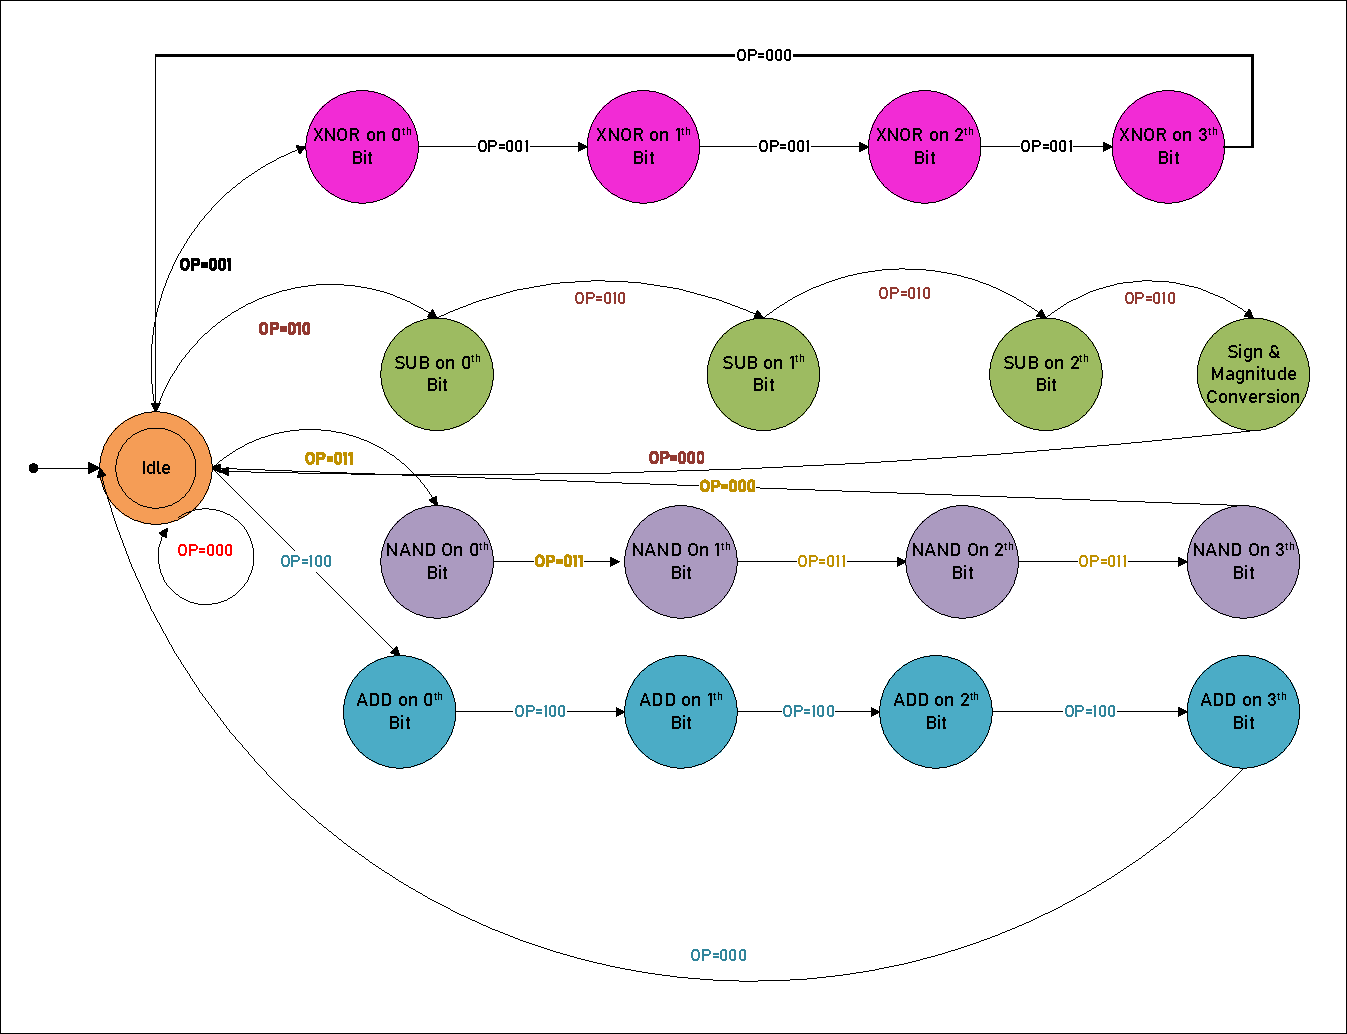
\includegraphics[height=6cm,width=6cm]{figures/FSM}}
    \caption{FSM Diagram}
    \label{fig:FSM}
\end{figure}

\begin{itemize}
    \item State 0 (\textit{2'b00}): In this state, the circuit performs the selected operation on the first bit of the input values and transitions to the next state.
    \item State 1 (\textit{2'b01}): In this state, the circuit performs the selected operation on the second bit of the input values and transitions to the next state.
    \item State 2 (\textit{2'b10}): In this state, the circuit performs the selected operation on the third bit of the input values and transitions to the next state.
    \item State 3 (\textit{2'b11}): In this state, the circuit performs the selected operation on the fourth and most significant bit of the input values and transitions back to the initial state.
\end{itemize}

Before transition, it also sets the values of \textit{zero} flag, \textit{sign} flag and \textit{carry} flag.


Things are checked and done slightly different based on the \textit{opcode}.
It can be observed from the above Fig \ref{fig:FSM} clearly.
The four different operations are implemented using a \textit{case} statement with \textit{opcode} as the selector.
Each operation \textit{case} statement contains the logic required to perform the operation on the given input values,
and update the output values of the circuit accordingly.
For example, for the \textbf{ADD} operation, the code first calculates the SUM of the LSBs of the input values,
adds the carry value to it (initially 0),
and assigns the SUM and the carry value to the output register \textbf{C}.
Then, it updates the \textit{zero} flag, which is set to 1 if the output is 0,
and transitions to the next state which is \textbf{IDLE} state that we can see from Figure \ref{fig:FSM}.
The outputs of the circuit include \textbf{C}, which stores the result of the operation,
\textit{carr}, which is the \textbf{carry} bit generated during addition or subtraction,
\textit{sign}, which is the sign bit of the output value, and zero, which is set to 1 if the output is \textit{0000}.
Overall, the FSM implementation allows the circuit to perform different arithmetic and logical
operations on the given input values, and update the output values based on the operation performed.